\documentclass[10pt]{article}
\usepackage{a4}
\usepackage{epsfig}
\usepackage{listings}
\usepackage{tabularx}
\lstset{language=Delphi}%
\lstset{basicstyle=\sffamily\small}%
\lstset{commentstyle=\itshape}%
\lstset{keywordstyle=\bfseries}%
\lstset{blankstring=true}%
\newcommand{\file}[1]{\textsf{#1}}
\usepackage[pdftex]{hyperref}
\newif\ifpdf
\ifx\pdfoutput\undefined
  \pdffalse
\else
  \pdfoutput=1
  \pdftrue
\fi
\begin{document}
\title{Programming GTK in Free Pascal: Making a real-world application.}
\author{Florian Kl\"ampfl\\and\\Micha\"el Van Canneyt}
\date{January 2001}
\maketitle
\section{Introduction}
In the third article on programming the GTK toolkit, the use of several
GTK widgets is demonstrated by building a real-world application. 

The main widgets to be shown are the Toolbar, CList and Tree widgets. 
Along the way, some other widgets such as a dialog will be shown as well.

The program to show all this will be a small file explorer. It will not
perform all functions that one would expect from a file explorer, but it
is not meant to be, either. It just demonstrates how one could go about when
making a file explorer. 

The File explorer will have 2 main components. One is a directory tree
which can be used to select a directory. the other is a Clist, a component
that presents a list of items in a table with headings. The Clist will be
used to display the files in the directory selected in the directory tree.

The functionality included will be limited to viewing the properties of
a file, and deleting a file. The view can be customized, and sorting of
columns by clicking the column header is possible.

Each window developed in the article will be described in a record, i.e.
all window elements will have a field in a record that points to the 
GTK widget used. Several forms will be developed, and each form will be
put in a separate unit. Signal callbacks will in general receive a
'userdata' pointer that points to the window record. This approach mimics
the object oriented approach of GTK, and is similar to the approach in
Delphi, where instead of a object, a window class is used.

\section{The main window}
The main window will consist of a menu, a tool bar, a directory tree and
the file list. The bottom of the screen will contain a statusbar. Between
the directory tree and the file list is a splitter that can be used to
resize the directory tree.

Right-clicking on the file list will show a popup menu, from which file
actions can be selected.

All the widgets in the main window will be stored in a big record
\lstinline|TMainWindow|:
\begin{lstlisting}{}
  TMainWindow = Record
    FDir,
    FMask : String;
    Window : PGtkWindow;
    Menu : PGtkMenuBar;
    Toolbar : PGtkToolBar;
    DirTree : PGtkTree;
    FileList : PGtkClist;
    Pane : PGtkPaned;
    StatusBar : PGtkStatusBar;
    FilesHeader,DirHeader : PGtkLabel;
    // helper objects - Menu
    Accel : PGtkAccelGroup;
    MFile,
    MView,
    MColumns,
    MHelp,
    // Main menu items
    PMFiles : PGtkMenu;
    MIFile,
    MIFileProperties,
    MIFileDelete,
    MIExit,
    MiColumns,
    MIAbout,
    MIHelp : PGtkMenuItem;
    MIShowTitles,
    MIShowExt,
    MIShowSize,
    MiShowDate,
    MIShowAttrs : PGtkCheckMenuItem;
    // Files PopupMenu Items:
    PMIFileProperties,
    PMIFileDelete : PGtkMenuItem;
    // Packing boxes
    VBox,
    LeftBox,
    RightBox : PGtkBox;
    // Scroll boxes
    TreeScrollWindow,
    ListScrollWindow : PGtkScrolledWindow;
    // Tree root node.
    RootNode : PGtkTreeItem;
  end;
  PMainWindow = ^TMainWindow;   
\end{lstlisting}
The record resembles a form class definition as used in \lstinline|Delphi|, it
contains all possible widgets shown on the window.

The most important ones are of course the \lstinline|DirTree| and \lstinline|FileList|
fields, the \lstinline|Menu| which will refer to the main menu and the
\lstinline|PMfiles| which will hold the popup menu. The Status bar is of course
in the \lstinline|StatusBar| field, and the \lstinline|ToolBar| field will hold the main
toolbar of the application. 

The \lstinline|FDir| field will be used to hold the currently shown 
directory and the \lstinline|FMask| field can be used to store a file mask that
determines what files will be shown in the list.

All these fields are filled in using the function \lstinline|NewMainForm| :
\begin{lstlisting}{}
Function NewMainForm : PMainWindow;
\end{lstlisting}

The function starts as follows :
\begin{lstlisting}{}
begin
  Result:=New(PMainWindow);
  With Result^ do
    begin
    FMask:='*.*';
    Window:=PgtkWindow(gtk_window_new(GTK_WINDOW_TOPLEVEL));
    gtk_window_set_title(Window,SFileExplorer);
    gtk_widget_set_usize(PgtkWidget(Window),640,480);
    gtk_signal_connect (PGTKOBJECT (window), 'destroy',
                    GTK_SIGNAL_FUNC (@destroy), Result);
    gtk_widget_realize(PgtkWidget(window)); 
\end{lstlisting}
This is a more or less standard GTK setup for a window. Note that the
pointer to the window record is passed to the 'destroy' signal handler
for the window, and that the window widget is realized (so a actual 
window is created). The necessity for the 'realize' call is explained below.

After the window is created, the main widgets on the form are created:
\begin{lstlisting}{}
Menu:=NewMainMenu(Result);
ToolBar:=NewToolbar(Result);
StatusBar:=PgtkStatusBar(gtk_statusbar_new);
FileList:=NewFileList(Result);
DirTree:=NewDirtree(Result);
PMFiles:=NewFilePopupMenu(Result);
\end{lstlisting}

The functions used to create these widgets will be discussed further on.
\begin{description}
\item[Menu] The menu is created in the function \lstinline|NewMainMenu|
\item[ToolBar] The toolbar is created in the \lstinline|NewToolbar| function.
\item[FileList] The CList component which will show the file data. Created
using \lstinline|NewFileList|.
\item[DirTree] The directory tree showing the directory structure of the
disk is created using \lstinline|NewDirtree|.
\item[PMFiles] is the popup menu for the file list and is created in the
\lstinline|NewFilePopupMenu| function.
\end{description}
Each function will set the fields which contain the helper widgets.

After the main widgets have been created, it is time to put them on the
form, and the rest of the \lstinline|NewMainForm| function is concerned 
mainly with  placing the widgets in appropriate containers. 

A splitter widget in GTK is called a \lstinline|paned window|. It can be created
using one of the following functions:
\begin{lstlisting}{}
function gtk_hpaned_new : PGtkWidget;
function gtk_vpaned_new : PGtkWidget;
\end{lstlisting}
Since the directory tree and file explorer window will be located left to
each other, a \lstinline|gtk_hpaned_new| call is needed for the file explorer.

The \lstinline|paned window| has 2 halves, in each of which a widget can be
placed. This is done using the following calls:
\begin{lstlisting}{}
procedure gtk_paned_add1(paned:PGtkPaned; child:PGtkWidget);cdecl;
procedure gtk_paned_add2(paned:PGtkPaned; child:PGtkWidget);cdecl;
\end{lstlisting}
The first function adds a widget to the left pane, the second to the right
pane (or the top and bottom panes if the splitter is vertical).

With this knowledge, the Directory Tree and File List can be put on the
form. In the case of the file explorer, 2 widgets will be packed in vertical
boxes which are on their turn put the left and right panes of the splitter: 
\begin{lstlisting}{}
Pane:=PgtkPaned(gtk_hpaned_new);
DirHeader:=PgtkLabel(gtk_label_new(pchar(SDirTree)));
LeftBox:=PGtkBox(gtk_vbox_new(false,0));
gtk_box_pack_start(Leftbox,PGtkWidget(DirHeader),False,False,0);
gtk_box_pack_start(Leftbox,PgtkWidget(TreeScrollWindow),true,True,0);
gtk_paned_add1(pane,PGtkWidget(Leftbox));
\end{lstlisting}
The left-hand side vertical box (\lstinline|LeftBox|) contains a label 
(\lstinline|DirHeader|) which serves as a  heading for the directory tree (\lstinline|DirTree|). 
It displays a static text (in the constant \lstinline|SDirTree|).

The right pane can be filled in a similar way with the file list:
\begin{lstlisting}{}
FilesHeader:=PgtkLabel(gtk_label_new(pchar(SFilesInDir)));
RightBox:=PGtkBox(gtk_vbox_new(false,0));
gtk_box_pack_start(Rightbox,PGtkWidget(FilesHeader),False,False,0);
gtk_box_pack_start(Rightbox,PGtkWidget(ListScrollWindow),true,True,0);
gtk_paned_add2(pane,PGtkWidget(Rightbox));
\end{lstlisting}
The right-hand side vertical box contains a label \lstinline|FileHeader| 
which serves as a heading for the file list (\lstinline|FileList|). 
It will be used to display the current directory name 
(\lstinline|SFilesInDir| constant).

After the directory tree and file view have been put in a paned window,
all that is left to do is to stack the statusbar, paned window, toolbar 
and menu in a vertical box \lstinline|VBox| which covers the whole window:
\begin{lstlisting}{}
  VBox:=PGtkBox(gtk_vbox_new(false,0));
  gtk_container_add(PGtkContainer(Window),PgtkWidget(VBox));
  gtk_box_pack_start(vbox,PGtkWidget(Menu),False,False,0);
  gtk_box_pack_start(vbox,PGtkWidget(ToolBar),False,False,0);
  gtk_box_pack_start(vbox,PGtkWidget(Pane),true,true,0);
  gtk_box_pack_start(vbox,PGtkWidget(StatusBar),false,false,0);
  gtk_widget_show_all(PGtkWidget(vbox));
  end;
end;
\end{lstlisting}
The destroy signal of the window does nothing except destroying the
main window record and telling GTK to exit the event loop:
\begin{lstlisting}{}
procedure destroy(widget : pGtkWidget ; Window : PMainWindow); cdecl;
begin
  gtk_clist_clear(Window^.FileList);
  dispose(Window);
  gtk_main_quit();
end;
\end{lstlisting}
The call to \lstinline|gtk_clist_clear| serves to clear the file list window.
The necessity for this call will be explained below.

\section{The file list}
The file list is constructed using the GTK CList widget. This is a powerful
widget that contains a lot of functionality, comparable to the
\lstinline|TListView| component found in Delphi.

A the file list  widget is created using the following function:
\begin{lstlisting}{}
Function NewFileList(MainWindow : PMainWindow) : PGtkClist;

Const 
  Titles : Array[1..6] of pchar = 
         ('Name','ext','Size','Date','Attributes','');

begin
  MainWindow^.ListScrollWindow:=
    PGtkScrolledWindow(gtk_scrolled_window_new(Nil,Nil));
  gtk_scrolled_window_set_policy(MainWindow^.ListScrollWindow,
                                 GTK_POLICY_AUTOMATIC,
                                 GTK_POLICY_AUTOMATIC);
  Result:=PGtkClist(Gtk_Clist_New_with_titles(6,@Titles));
  gtk_Container_add(PGTKContainer(MainWindow^.ListScrollWindow),
                    PGtkWidget(Result));
\end{lstlisting}
A Clist object is not capable of drawing scroll bars if it contains too many
items for its size, so first a \lstinline|Scrolled Window| is created in which
the Clist object is embedded. A scrolled window is a container widget which 
does nothing except providing scrollbars for the widget it contains.

A scrolled window is created using the \lstinline|gtk_scrolled_window_new|
function:
\begin{lstlisting}{}
function gtk_scrolled_window_new(hadjustment:PGtkAdjustment;
                                 vadjustment:PGtkAdjustment):PGtkWidget
\end{lstlisting}
The \lstinline|Adjustment| parameters can be used to pass scrollbar widgets
that the scrolled window should use to do it's work.
If none are passed, the scrolled window will create the needed scrollbars
by itself.

The visibility of the scrollbars can be controlled with the policy property
of the scrolled window:
\begin{lstlisting}{}
gtk_scrolled_window_set_policy(scrolled_window:PGtkScrolledWindow;
                               hscrollbar_policy:TGtkPolicyType; 
                               vscrollbar_policy:TGtkPolicyType)
\end{lstlisting}
The horizontal and vertical policies can be set to the following values:
\begin{description}
\item[GTK\_POLICY\_AUTOMATIC] Scrollbars are only visible if they are needed.
\item[GTK\_POLICY\_ALWAYS] Scrollbars are always visible.
\end{description}

After the creation of the scrolled window, the file list is created and
added to the scrolled window. A CList widget can be created using 2 calls;
\begin{lstlisting}{}
function  gtk_clist_new (columns:gint):PGtkWidget;
function  gtk_clist_new_with_titles (columns:gint;
                                     titles:PPgchar):PGtkWidget;
\end{lstlisting}
In both cases, the number of columns in the list must be passed. If
the column header titles are fixed and known, they can be passed in the
\lstinline|gtk_clist_new_with_titles| call, but they can still be set and
retrieved later on with the following calls:
\begin{lstlisting}{}
Procedure gtk_clist_set_column_title(clist:PGtkCList;
                                     column:gint;
                                     title:Pgchar);cdecl;
function  gtk_clist_get_column_title(clist:PGtkCList;
                                     column:gint):Pgchar;cdecl;
\end{lstlisting}
Note that the column indices are 0 based.

After the CList widget has been created, some properties can be set:
\begin{lstlisting}{}
gtk_clist_set_shadow_type(Result,GTK_SHADOW_ETCHED_OUT);
\end{lstlisting}
This call sets the border around the clist. The possible values for
the last parameter (the \lstinline|TGtkShadowType|) of 
\lstinline|gtk_clist_set_shadow_type| are:
\begin{description}
\item[GTK\_SHADOW\_NONE] No border.
\item[GTK\_SHADOW\_IN] the clist appears lowered.
\item[GTK\_SHADOW\_OUT] the clist appears raised.
\item[GTK\_SHADOW\_ETCHED\_IN] the clist appears with a lowered frame.
\item[GTK\_SHADOW\_ETCHED\_OUT] the clist appears with a raised frame.
\end{description}

The justification of a column in the list can be set:
\begin{lstlisting}{}
gtk_clist_set_column_justification(result,2,GTK_JUSTIFY_RIGHT);
\end{lstlisting}
column 2 will contain the file sizes, so it is set right-justified.
Other possible values are for justification are 
\lstinline|GTK_JUSTIFY_LEFT|, \lstinline|GTK_JUSTIFY_CENTER|, and 
\lstinline|GTK_JUSTIFY_FILL|,  which have their obvious meanings.

To be able to select multiple items (or rows) at once, the selection mode of
the CList must be set: 
\begin{lstlisting}{}
gtk_clist_set_selection_mode(Result,GTK_SELECTION_MULTIPLE);
\end{lstlisting}
Possible modes of selection are:
\begin{description}
\item[GTK\_SELECTION\_SINGLE] Only one row can be selected at any given
time.
\item[GTK\_SELECTION\_BROWSE] Multiple items can be selected, however the
selection will always return 1 item.
\item[GTK\_SELECTION\_MULTIPLE] Multiple items can be selected, and the
selection will contain all selected items.
\item[GTK\_SELECTION\_EXTENDED] The selection is always \lstinline|Nil|.
\end{description}
The selection is a field (\lstinline|selection|) of type \lstinline|PGList| in the 
\lstinline|TGtkCList| record. A \lstinline|PGlist| is a pointer to a doubly linked 
list with data pointers. More details about this will follow.

The elements in the list list can be sorted. 
\begin{lstlisting}{}
gtk_clist_set_auto_sort(Result,True);
If DefCompare=Nil then
  DefCompare:=Result^.compare; 
gtk_clist_set_compare_func(Result,
                           TGtkCListCompareFunc(@FileCompareFunc));
\end{lstlisting}
By default, a CList sorts by comparing the texts in the current sort column 
of the items in the list. This sorting happens using the \lstinline|compare| 
function of the CList. The standard \lstinline|compare| function of the list 
is saved here in a variable \lstinline|DefCompare|, so it can still be used. 
Using the  \lstinline|gtk_clist_set_compare_func| the compare function to be 
used when sorting can be set, and it is set to the function 
\lstinline|FileCompareFunc|,  which will be discussed later on.

The \lstinline|gtk_clist_set_auto_sort| can be used to set the auto-sort
feature of the Clist. If auto-sort is on, adding new items to the CList will
insert them in the correct order. If auto-sort is off, new items are
appended to the beginning or end of the list.

After the sort function is set, handlers are attached to 2 signals:
\begin{lstlisting}{}
gtk_signal_connect(PgtkObject(Result),'button_press_event',
                   TGtkSignalFunc(@ShowPopup),MainWindow);
gtk_signal_connect(PgtkObject(Result),'click_column',
                   TGtkSignalFunc(@FileColumnClick),MainWindow);
\end{lstlisting}
The first handler connects to a mouse button press event. This will be used
to detect a right mouse click, and to show a popup menu:
\begin{lstlisting}{}
Procedure ShowPopup(Widget : PGtkWidget; 
                    Event : PGdkEventButton; 
                    Window : PMainWindow);cdecl;

begin
  if (event^.thetype=GDK_BUTTON_PRESS) and 
     (event^.button=3) then
    gtk_menu_popup(Window^.PMFiles,Nil,Nil,Nil,NIl,3,event^.time);
end;
\end{lstlisting}
The \lstinline|gtk_menu_popup| function does nothing but showing the menu;
when a menu item is clicked, the menu will close by itself.

The second handler connects to the 'click\_column' event. This event is
emitted if the user clicks on the column header. It will be used to switch
the sort order of the file list:
\begin{lstlisting}{}
Procedure FileColumnClick(List : PGtkCList;Column:gint; Window : PMainWindow);cdecl;

Var 
  I  : longint;
  NS : TGtkSortType;
   
begin
  If Column<>List^.sort_column Then
    begin
    gtk_clist_set_sort_type(List,GTK_SORT_ASCENDING);
    gtk_clist_set_sort_column(list,Column);
    end
  else
    begin
    If (List^.Sort_type=GTK_SORT_ASCENDING) Then 
      NS:=GTK_SORT_DESCENDING
    else
      NS:=GTK_SORT_ASCENDING;
    gtk_clist_set_sort_type(List,NS);
    end;
  gtk_clist_sort(list);
end;
\end{lstlisting}
The function starts by retrieving the current sort column. If it is
different from the column the used clicked on, then 2 things are done:
\begin{enumerate}
\item The sort type is set to ascending.
\item The sort column is set to the column the user clicked.
\end{enumerate}
If, on the other hand, the user clicks on a column that is the sort column, 
the sort type is simply reversed. After the sort column and sort type are 
set, the list is epxlicitly sorted. (neither of the calls that set the sort 
order or sort column forces a sort).

The sort happens using the \lstinline|compare| function (\lstinline|FileCompareFunc|)
that was set when the CList was created:
\begin{lstlisting}{}
Function FileCompareFunc(List:PGtkCList; Row1,Row2 : PGtkCListRow) : Longint; Cdecl;

Var 
  SC : Longint;

begin
  SC:=List^.sort_column;
  If SC in [2,3] then
    begin
    SC:=SC-2;
    Result:=PLongint(Row1^.Data)[SC]-PLongint(Row2^.Data)[SC];
    end
  Else
    Result:=DefCompare(List,Row1,Row2);  
end;
\end{lstlisting}
This function receives 3 arguments:
\begin{itemize}
\item The list that needs to be sorted.
\item 2 pointers to the row objects that must be compared.
\end{itemize}
The result must be an integer that is negative if the first row should come
before the second or larger than zero if the second row should come before
the first. If the result is zero then the columns are considered the same.

The function checks what the sort column is. If it is not the size (2) or 
date (3) column, then the default row compare function (which was saved in 
the \lstinline|DefCompare| variable when the list was created) is used to
compare the rows. If the size or date columns must be compared, the user 
data associated with the rows is examined. As will be shown below, the user
data will point to an array of 2 Longint values that describe the size and
datestamp of the file. The approriate values are compared and the result is 
passed back.

To fill the file list with data, the \lstinline|FillList| function is 
implemented:
\begin{lstlisting}{}
Function FillList(List : PGtkCList; 
                  Const Dir,Mask : String) : Integer;

Var
  Info : TSearchRec;
  Size : Int64;
  I,J : longint;
  
begin
  Result:=0;
  Size:=0;
  gtk_clist_freeze(List);
  Try
    gtk_clist_clear(List);
    If FindFirst (AddTrailingSeparator(Dir)+Mask,
                  faAnyFile,Info)=0 then
      Repeat
        Inc(Size,Info.Size);
        AddFileToList(List,Info);
        Inc(Result);
      Until FindNext(Info)<>0;
    FindClose(info);
  finally
    For I:=0 to 4 do
      begin
      J:=gtk_clist_optimal_column_width(List,i);
      gtk_clist_set_column_width(List,i,J);
      end;
    gtk_clist_thaw(List)
  end;
end;
\end{lstlisting}
This function is very straightforward. To start, it 'freezes' the list with
\lstinline|gtk_clist_freeze|; this prevents the list from updating the
screen each time a row is added or deleted. Omitting this call would cause
serious performance degradation and screen flicker.

After freezing the list, it is cleared; Then a simple loop is implemented
that scans the given directory with the given file mask using the
\lstinline|FindFirst|/\lstinline|FindNext| calls. For each file found
it calls the \lstinline|AddFileToList| function, that will actually add the
file to the list view, using the information found in the search record.

The \lstinline|AddTrailingSeparator| adds a directory separator to a 
string containing the name of a directory if this does not end on a 
separator yet. It can be found in the \file{futils} unit.

After the loop has finished, the optimal width for each column is 
retrieved using the \lstinline|gtk_clist_optimal_column_width| function
and the result is used to set the column width. As a result, the columns will
have the correct size for displaying all items.

When this has been done, the list is 'thawed' with \lstinline|gtk_clist_thaw|,
which means that it will repaint itself if needed. This happens in a 
\lstinline|finally| block since the \lstinline|gtk_clist_freeze| and 
\lstinline|gtk_clist_thaw| work with a reference counter. For each 'freeze' 
call the counter is increased. It is decreased with a 'thaw' call. When the
counter reaches zero, the list is updated.

The function that actually adds a row to the list view is quite simple:
\begin{lstlisting}{}
Procedure AddFileToList(List : PGtkCList; Info : TSearchRec);

Var
  Texts : Array[1..6] of AnsiString;
  FSD   : PLongint;
  I     : longint;
      
begin
  Texts[1]:=ExtractFileName(Info.Name);
  Texts[2]:=ExtractFileExt(Info.Name);
  Texts[3]:=FileSizeToString(Info.Size);
  Texts[4]:=DateTimeToStr(FileDateToDateTime(Info.Time));
  Texts[5]:=FileAttrsToString(Info.Attr);
  Texts[6]:='';
  i:=gtk_clist_append(List,@Texts[1]);
  FSD:=GetMem(2*SizeOf(Longint));
  FSD[0]:=Info.Size;
  FSD[1]:=Info.Time;
  gtk_clist_set_row_data_full (List,I,FSD,@DestroySortData);
end;
\end{lstlisting}
The \lstinline|gtk_clist_append| call accepts 2 paramers: a CList, and a
pointer to an array of zero-terminated strings. The array must contain as
much items as the CList has columns (in the above, the last column is 
always empty, as this gives a better visual effect). The call adds a column
at the end of a list; An item can be inserted at the beginning of the list
with \lstinline|gtk_clist_append|, which accepts the same parameters. An
item can be inserted at certain position:
\begin{lstlisting}{}
gtk_clist_insert(clist:PGtkCList; row:gint; thetext:PPgchar);cdecl;
\end{lstlisting}
Note that all these calls do the same thing if the 'auto sort' was set for
the CList.

The \lstinline|FileAttrsToString| function converts file attributes to a
string of characters that indicate whether a given attribute is present.
It can be found in the \file{futils} unit and will not be shown here.

After the file data was appended to the CList, an array of 2 longints is
allocated on the heap. The first longint is filled with the size of the
file, the second with the date of the file. The pointer to this array is
then associated with the row that was just inserted with the
\lstinline|gtk_clist_set_row_data_full| call. There are 2 calls to
associate data with a row:
\begin{lstlisting}{}
gtk_clist_set_row_data(clist:PGtkCList; 
                       row:gint; 
                       data:gpointer);cdecl;
gtk_clist_set_row_data_full(clist:PGtkCList; 
                            row:gint; data:gpointer; 
                            destroy: :TGtkDestroyNotify);
\end{lstlisting}
the first call is used to add data to a clist that will not need to be
destroyed if the row is deleted. The second call can be used to pass a
callback that will be called when the row is destroyed. 

In the case of the file list, the \lstinline|DestroySortData| call is
used to dispose the array with sort data:
\begin{lstlisting}{}
Procedure DestroySortData(FSD : Pointer);cdecl;
 
begin
  FreeMem(FSD);
end;                                                                            
\end{lstlisting}
The reason that the file list is cleared when the main window is destroyed
now becomes apparent: when the list is cleared, all data associated with
the file list is freed. If the call to \lstinline|gtk_clist_clear| is
omitted before destroying the main window, the list is not cleared and all
data stays in memory even after the window closes.

The display of the column titles of the file list can be switched on or off.
To do this a check menu item ('Hide titles') is added to the 'View' menu. 
If the menu is clicked, the following callback is executed:
\begin{lstlisting}{}
Procedure ToggleFileListTitles(Sender : PGtkCheckMenuItem;
                               Window : PMainWindow);cdecl;

begin
  If active(Sender^)=0 then
    gtk_clist_column_titles_show(Window^.FileList)
  else  
    gtk_clist_column_titles_hide(Window^.FileList)
end;
\end{lstlisting}
The \lstinline|active| function checks whether a check menu item is currently 
checked ot not and shows or hides the titles. 

Not only can the column titles be switched on or off, it is also possible to
control whether or not a given column must be shown;

Under the 'View' menu, there is a 'Hide columns' submenu that contains 4
check menus that can be used to toggle the visibility of the columns in the
file list. All the check menu items are connected to the following callback:
\begin{lstlisting}{}
Procedure ToggleFileListColumns(Sender : PGtkCheckMenuItem;
                                Window : PMainWindow);cdecl;

Var Col : Longint;

begin
  With Window^ do
    If Sender=MIShowExt Then
      Col:=1
    else if Sender=MiShowSize Then
      Col:=2
    else if Sender=MIShowDate then
      Col:=3
    else 
      Col:=4;
   gtk_clist_set_column_visibility(Window^.FileList,
                                   Col,
                                   (Active(Sender^)=0));   
end;
\end{lstlisting}
The call gets as 'user data' a pointer to the main window record. Using this
it checks which menu emitted the call, and updates the corresponding column
with the \lstinline|gtk_clist_set_column_visibility| function.

More attributes of a CList can be set, but they will not be discussed here; 
the GTK documentation and tutorial offer an overview of the possibilities. 

The selection mode of the CList has been set to allow selection of multiple
rows. The Clist maintains a linked list (A Glist) with the rows that are
part of the selection. The linked list contains the indexes of the selected
rows in it's associated data.

The linked list \lstinline|Glist| is often used in GTK applications. 
It consists of the  following records:
\begin{lstlisting}{}
TGList = record
  data gpointer;
  next,prev : PGlist;
end;
PGlist=^TGlist;
\end{lstlisting}
The selection of a CList is of type \lstinline|PGlist|. The \lstinline|data|
pointer can be typecasted to an integer to return the index of a selected
row.

The following function walks the selection linked list and stores the
associated filenames in a \lstinline|TStrings| class:
\begin{lstlisting}{}
Procedure GetFileSelection (List : PGtkClist; Selection : TStrings);

Var
  SList : PGList;
  Index : Longint;
  P : PChar;
  
begin
  Selection.Clear;
  Slist:=List^.Selection;
  While SList<>nil do
    begin
    Index:=Longint(SList^.Data);
    gtk_clist_get_text(List,Index,0,@p);
    Selection.Add(StrPas(p));
    SList:=g_list_next(SList);
    end;
end;
\end{lstlisting}
The \lstinline|gtk_clist_get_text| retrieves the text of a given cell in the
CList (a similar function exists to set the text) , and the
\lstinline|g_list_next| jumps to the next element in the linked list.

The \lstinline|TStrings| class is the standard string container as defined
in the \lstinline|Classes| unit of Free Pascal (or Delphi).

The above function will be used to retrieve the list of selected files so
operations can be done on the selection.

To retrieve the first (and possibly only) item of a selection, and the
number of items in a selection, the following functions can be used:
\begin{lstlisting}{}
Function GetFileFirstSelection (List : PGtkClist) : String;

Var
  SList : PGList;
  Index : Longint;
  P : PChar;
  
begin
  Result:='';
  Slist:=List^.Selection;
  If SList<>nil then
    begin
    Index:=Longint(SList^.Data);
    gtk_clist_get_text(List,Index,0,@p);
    Result:=StrPas(p);
    end;
end;

Function GetFileSelectionCount (List : PGtkClist) : Longint;

Var
  SList : PGList;
  
begin
  Slist:=List^.Selection;
  Result:=0;
  While SList<>nil do
    begin
    Inc(Result);
    SList:=g_list_next(SList);
    end;
end;
\end{lstlisting}
These functions will be used further on.

The filelist is now ready to be used. To be able to select a directory from
which the files should be displayed, a Tree widget is used. How to create
this tree and connect it to the file list is explained in the next section.

\section{The directory tree}
The directory tree will allow the user to browse through the directories on
his system. When a directory is selected, the file view should be updated 
to show the files in the selected directory.

To make the directory tree more efficient and less memory consuming, the
tree is not filled with the whole directory tree at once. Instead, only 2
levels of directories will be put in the tree. The tree is progessively
filled as the user expands the directory nodes. 

The directory tree is created in the following function:
\begin{lstlisting}{}
Function NewDirtree (MainWindow : PMainWindow) : PGtkTree;
 
begin
  Result:=PGtkTree(gtk_tree_new());
  With MainWindow^ do
    begin
    TreeScrollWindow:=PGtkScrolledWindow(gtk_scrolled_window_new(Nil,Nil));
    gtk_widget_show(PGtkWidget(TreeScrollWindow));
    gtk_scrolled_window_set_policy(TreeScrollWindow,
                                 GTK_POLICY_AUTOMATIC,
                                 GTK_POLICY_AUTOMATIC);
    gtk_scrolled_window_add_with_viewport(TreeScrollWindow,PGtkWidget(Result));
    RootNode:=PGtkTreeItem(gtk_tree_Item_new_with_label(Pchar(PathSeparator)));
    gtk_tree_append(Result,PgtkWidget(RootNode));
    scandirs(PathSeparator,Result, RootNode,True,MainWindow);
    gtk_tree_item_expand(rootnode);
    end;
end;                                                                            
\end{lstlisting}
The function starts off by creating the tree widget which is the return
value of the function.

Similar to the Clist, the tree widget does not possess functionality 
for displaying scroll bars, so a 'scrolled window' is created, 
in which the tree widget is placed. 

A tree can have one or more tree items connected to it. Each of these tree
items can in turn have a tree associated with it, which in turn can again
have tree items associated. This way the tree is recursively constructed.

The directory tree is filled with 1 tree item, which will represent the root
directory of the disk which is browsed with the file explorer; The
\lstinline|gtk_tree_item_new_with_label| call returns a new tree item,
which is then appended to the tree using the \lstinline|gtk_tree_append|
call.

After this is done, the directories below the root directory are scanned and
appended to the root node in the \lstinline|scandirs| function, explained
below. If the root node was filled, then it is expanded with
\lstinline|gtk_tree_item_expand| (it can be collapsed with
\lstinline|gtk_tree_item_collapse|)

The \lstinline|scandirs| function scans a given directory for subdirectories
and appends each directory to a subtree of a given node. The subtree is
created if needed:
\begin{lstlisting}{}
Procedure Scandirs(Path: String; Tree : PgtkTree;
                   Node: PGtkTreeItem ; SubSub : Boolean;
                   Window : PMainWindow);

Var
  NewTree : PGtkTree;
  NewNode : PGtkTreeItem;
  Info : TSearchRec;
  S,FP : AnsiString;

begin
  NewTree:=Nil;
  FP:=AddTrailingSeparator(Path);
  If FindFirst(FP+'*.*',faAnyfile,Info)=0 then
    Try 
      repeat
        If ((Info.Attr and faDirectory)=faDirectory) then
          begin
          S:=Info.Name;
          If (S<>'.') and (S<>'..') then
            begin
            If (Node<>Nil) then
              begin
              If (NewTree=Nil) and (node<>Nil) then
                begin
                NewTree:=PGtkTree(gtk_tree_new);
                gtk_tree_item_set_subtree(Node,PGtkWidget(NewTree));
                end
              end
            else
              NewTree:=Tree;                
            NewNode:=PGtkTreeItem(gtk_tree_item_new_with_label(Pchar(S)));
            gtk_tree_append(NewTree,PgtkWidget(NewNode));
            gtk_signal_connect(PGtkObject(NewNode),'select',
                               TGtkSignalFunc(@DirSelect),Window);
            gtk_signal_connect(PGtkObject(NewNode),'expand',
                               TGtkSignalFunc(@DirExpand),Window);
            If SubSub then 
              ScanDirs(FP+S,Tree,NewNode,False,Window);
            gtk_widget_show(PGtkWidget(NewNode));
            end;
          end;  
      until FindNext(Info)<>0;
    Finally 
      FindClose(Info);
    end;
  gtk_widget_show(PGtkWidget(Node));
end;    
\end{lstlisting}
The routine is a simple loop. If a subdirectory is found then a new 
tree widget is created (\lstinline|newTree|) and appended to the 
given node with the \lstinline|gtk_tree_item_set_subtree| call.

For each found subdirectory a new treeitem is created and appended to 
the subtree. 2 signals handlers are connected to the created tree item,
one for 'select' signal which is emitted when the user selects a tree item, 
and one for the 'expand' signal which is emitted when the user expands a 
node. Each of these handlers gets as data a pointer to the main window
record.
 
The \lstinline|SubSub| parameter is used to control the recursive behaviour.
If it is set to \lstinline|True|, the \lstinline|Scandirs| function will
call itself recursively, but only once. As a result only 2 levels of
subdirectories are scanned. 

Finally, the created nodes are shown.

When the user expands a node, the \lstinline|DirExpand| function is
called:
\begin{lstlisting}{}
Procedure DirExpand(Item : PGtkTreeItem; Window : PMainWindow);cdecl;
 
Var 
  Dir : String;
  SubTree : PGtkTree;
  SubNodes : PGList;
  Node : PGtkTreeItem;
   
begin
  SubTree:=PgtkTree(Item^.SubTree);
  SubNodes:=gtk_container_children(PGtkContainer(SubTree));
  While SubNodes<>Nil do
    begin
    Node:=PgtkTreeItem(SubNodes^.Data);
    If (Node^.SubTree<>Nil) then 
      gtk_tree_item_remove_subtree(Node);
    Scandirs(GetPathName(Node),Nil,Node,False,Window);
    SubNodes:=g_list_remove_link(SubNodes,SubNodes);
    end;
end;
\end{lstlisting}
The function starts by retrieving the subtree of the tree item that
triggered the callback. It then retrieves the list of subnodes (treeitems)
of the subtree which represent the subdirectories of the directory node 
that is about to be expanded. The Tree object descends from the GTK
container object, and keeps its treeitems in the container's children
list. This list is a Glist. The \lstinline|gtk_container_children| returns
a copy of the list containing the children.

Then a simple loop is executed: for each of
the found nodes, the subtree is destroyed if it exists:
\lstinline|gtk_tree_item_remove_subtree| removes a subtree from a treeItem
and destroys it. 

After the subtree is destroyed, at the subirectory is scanned for possible
subdirecties (remark that the \lstinline|SubSub| parameter is set to 
\lstinline|false|) and the subtree is recreated if needed.

The directory corresponding to a given node is calculated in the 
\lstinline|GetPathName| function, explained below.

The next cycle of the loop is started by removing and destroying the first
element of the GList with the \lstinline|g_list_remove_link| call:
the call returns the new start of the list with the element removed. By
passing the first element of the list as the element to be removed the 
whole list is traversed.

When the user selects a tree item, the list view must be updated with
the files in that directory. This is done in the \lstinline|DirSelect|
handler for the 'select' signal:
\begin{lstlisting}{}
Procedure DirSelect(Item : PGtkTreeItem; Window : PMainWindow);cdecl;
  
begin
  ShowDir(Window,GetPathName(Item));
end;

Procedure ShowDir (Window : PMainWindow; Dir : String);

begin
  With Window^ do
    begin
    FDir:=Dir;
    FillList(FileList,Dir,FMask);
    gtk_label_set_text(FilesHeader,pchar(Format(SFilesInDir,[Dir])));
    end;
end;

\end{lstlisting}
The \lstinline|Showdir| function will be called from other places as 
well hence it is put separately; The \lstinline|DirSelect| function
does nothing but to call the ShowDir function after it has calculated the
path of the treeitem that triggered the 'select' signal:
\begin{lstlisting}{}
Function GetPathName(Item : PGtkTreeItem) : String;

Var P : PChar;
    PTree : PGtkTree;
begin
  gtk_label_get(PgtkLabel(PGtkBin(Item)^.Child),@P);
  Result:=StrPas(P);
  If (PGtkWidget(item)^.Parent<>Nil) then
    begin
    PTree:=PGtkTree(PgtkWidget(Item)^.Parent);
    If (Ptree^.Level<>0) Then
      Result:=AddTrailingSeparator(GetPathName(PgtkTreeItem(PTree^.Tree_Owner)))+Result
    end;  
end;
\end{lstlisting}
It is a simple recursive mechanism. The only issue with this
routine is that one should know that the parent of a tree item is a tree,
and that the owner of the tree (in it's \lstinline|Tree_Owner| field) is 
in turn again a treeitem. The \lstinline|Level| field of a tree determines
at what level the tree is located (i.e. the number of nodes present above 
the tree) and can be used to check when the algorithm should stop.

An alternate approach would have been to associate with each node some 
user data, such as a string that is the full path name of the node.

With this, the tree is created and is linked to the file list, so the 
user has the capability to select any directory and display it's contents;
The user can also customize the view of the file list. 

However, no actions can be performed on the files. This is treated in the
next sections, where a toolbar and popup menu are used to allow the user to 
do things with the shown files.

\section{Adding a popup menu}
To allow the user to do something with the displayed files, a popup menu is
addd to the file list. Adding a popup menu is not different from adding a 
main menu to a form, just it will not be attached to a menu bar. The popup
menu will be hidden till the user right-clicks in the file list.

The popup menu is created in the following function:
\begin{lstlisting}{}
Function NewFilePopupMenu (MainWindow : PMainWindow) : PGtkMenu;

begin
  result:=PGtkMenu(gtk_menu_new);
  gtk_signal_connect(PGtkObject(result),'show',
                     TGtkSignalFunc(@PMFilesActivate),MainWindow);
  With MainWindow^ do
    begin
    PMIFileProperties:=AddItemToMenu(Result,Accel,'_Properties','',
                                     TgtkSignalFunc(@DoProperties),
                                      MainWindow);
    PMIFileDelete:=AddItemToMenu(Result,Accel,'_Delete','<ctrl>d',
                                 TgtkSignalFunc(@DeleteFile),
                                 MainWindow);
    end; 
end;
\end{lstlisting}
The \lstinline|AddItemToMenu| functions were developed in an earlier
articles, and have been collected in the 'menus' unit. 

The 'show' handler attached to the menu is used to set the state
of some of the menu items when the menu pops up:
\begin{lstlisting}{}
Procedure PMFilesActivate(Widget : PGtkWidget; Window : PMainWindow); cdecl;

Var State : TGtkStateType;

begin
  if GetFileSelectionCount(Window^.FileList)>1 then
    State:=GTK_STATE_INSENSITIVE
  else
    State:=GTK_STATE_Normal;
  gtk_widget_set_state(PgtkWidget(Window^.PMIFileProperties),State);
end;
\end{lstlisting}
When more than 1 file is selected in the file view, the properties menu item
is disabled. 

The popup menu will appear if the user clicks the right button in the file
list; The necessary event handler for that (\lstinline|ShowPopup|) was 
attached to the CList and discussed earlier on.

The delete menu item has the following 'click' handler:
\begin{lstlisting}{}
Procedure DeleteFile(Widget : PGtkWidget; Window : PMainWindow); cdecl;

Var i : longint;
    S : TStringList;
    
begin
  S:=TStringList.Create;
  Try
    GetFileSelection(Window^.FileList,S);
    For I:=0 to S.Count-1 do
      begin
      For I:=0 to S.Count-1 do
        SysUtils.DeleteFile(Window^.FDir+S[i]);
      end;
  Finally
    If S.Count>0 then
      RefreshFileView(Window);
    S.Free;
  end;        
end;
\end{lstlisting}
The routine simply retrieves the selection list and deletes all files
present in it; After that the file view is refreshed.

The properties popup menu action will be treated later on.

\section{Adding a toolbar}
The toolbar in the file explorer application will contain 2 buttons with
a pixmap on them; the pixmap will be loaded from data compiled into the
binary. The actions performed by the toolbar buttons will be the same as
the actions in the popup menu: show a file's properties and delete the file.

The creation of the toolbar for the file explorer program is done in the
following function:
\begin{lstlisting}{}
Function NewToolbar (MainWindow : PMainWindow) : PGtkToolbar;

begin
  Result:=pGtkToolBar(gtk_toolbar_new(GTK_ORIENTATION_HORIZONTAL,
                                      GTK_TOOLBAR_ICONS));
  gtk_toolbar_append_item(result,
                          Nil,
                          'File Properties',
                          nil,
                          CreateWidgetFromXPm(PgtkWidget(MainWindow^.Window),
                                              @PropertiesXPM),
                          TgtkSignalFunc(@DoProperties),
                          MainWindow);
  gtk_toolbar_append_item(result,
                          Nil,
                          'Delete File',
                          Nil,
                          CreateWidgetFromXPm(PgtkWidget(MainWindow^.Window),
                                              @DeleteXPM),
                          TgtkSignalFunc(@DeleteFile),
                          MainWindow);
end;
\end{lstlisting}
The \lstinline|gtk_toolbar_new| function creates a new toolbar. The first
argument to this call specifies the orientation for the toolbar. Possible
values for the orientation are:
\begin{description}
\item[GTK\_ORIENTATION\_HORIZONTAL] The toolbar is filled horizontally;
\item[GTK\_ORIENTATION\_VERTICAL] The toolbar is filled vertically;
\end{description}
The second argument determines the style of the toolbar; it can have the
following values:
\begin{description}
\item[GTK\_TOOLBAR\_TEXT] Toolbuttons just show a text.
\item[GTK\_TOOLBAR\_ICONS] Toolbuttons just show a pixmap.
\item[GTK\_TOOLBAR\_BOTH] toolbuttons show both a pixmap and text.
\end{description}
The style determines what widgets will be placed on new toolbuttons that
are added with the \lstinline|gtk_toolbar_append_item| or
\lstinline|gtk_toolbar_prepend_item| calls. If buttons are added to the 
toolbar manually, the style has no effect.

The \lstinline|gtk_toolbar_append_item| call adds a new toolbar button 
to the end of a toolbar. The \lstinline|gtk_toolbar_prepend_item| item 
inserts a new button at the beginning of the toolbar. Both accept the 
following arguments:
\begin{enumerate}
\item a pointer to the toolbar to which the item should be added.
\item a zero-terminated string with the text to be shown on the button.
\item a zero-terminated string with the tooltip text (the hint) for the button.
\item a zero terminated private tooltip text for the button.
\item an icon wiget, usually a GtkPixmap.
\item A callback function of type \lstinline|TGtkSignalFunc| that will be 
executed when the user clicks the button.
\item Callback data pointer which will be passed to the callback.
\end{enumerate}
A toolbutton can also be inserted at a certain position with the
\lstinline|gtk_toolbar_insert_item| call. It accepts an additional (last) 
argument, the position at which to insert the toolbutton. 

For the toolbar of the file explorer program, the buttons contain no text
(since the \lstinline|GTK_TOOLBAR_ICONS| style was chosen for the toolbar)
they do contain an icon, a pixmap widget.

The pixmap widget is created with the following function:
\begin{lstlisting}{}
function CreateWidgetFromXPM (Window : PGtkWidget; 
                              Data : PPChar) : PGtkWidget;

Var
  mask   : PGdkBitmap;
  pixmap : PGdkPixMap;

begin
  pixmap:=gdk_pixmap_create_from_xpm_d(window^.window,@mask,nil,ppgchar(Data));
  Result:=gtk_pixmap_new(Pixmap,Mask);
  gtk_widget_show(Result);
end;
\end{lstlisting}
This function accepts 2 arguments: A GTK window, and a pointer to an array
or zero-terminated strings which describe the pixmap. With these it creates 
a gdk pixmap object with the \lstinline|gdk_pixmap_create_from_xpm_d| call.
this function expects the following arguments:
\begin{enumerate}
\item A pointer to a GDK window object. In the above, the GDK window of the
main window widget is used. This explains why the \lstinline|gtk_widget_realize|
call was made when creating the main window: When the widget is realized, a
window is allocated to it. If the main window widget was not realized, then
it's gdk window would be nil.
\item The address of a \lstinline|PGdkBitmap| which will be used to store
the mask of the created pixmap. The mask determines the transparent items
in the bitmap, and can be used when creating a pixmap widget. This may be
nil.
\item A pointer to a color that should be considered the transparent
color. This may be nil, in which case a default color is used.
\item A pointer to a XPM pixmap structure. 
\end{enumerate}
After the GDK pixmap and the mask were created, a pixmap widget is created
from the GDK bitmap, and the widget is shown.

The pixmap data is in XPM format. The XPM format is an array of
zero-terminated strings which are organized as follows:
\begin{enumerate}
\item A string describing the pixmap dimensions and the number of colors.
The string is of the form 
\begin{verbatim}
'width height #colors chars/color',
\end{verbatim}
So the string
\begin{verbatim}
'16 16 4 1'
\end{verbatim}
means a 16x16 bitmap, using 4 colors, described by 1 character per color.
\item A series of strings that describe the color. the number of strings
should equal the count specified in the first string. The color descriptions
should have the following form:
\begin{verbatim}
'X c #YYYYYY'
\end{verbatim}
here 'X' must be replaced by N characters, where N is the number of
characters per color that was specified in the first string. The YYYYYY
is a RGB color value, in hex format. Each red,green or blue value must
contain 2 or 4 characters. The string '\#FF0000' would describe red, just as
'\#FFFF00000000' would describe red.

Instead of a rgb value, 'None' can be specified to indicate a transparent
color.
Some examples of valid colors would be:
\begin{verbatim}
'. c #000000',      { Black }
'# c #000080',      { Dark Blue }
'a c None',         { Transparent }
'b c #f8fcf8',      { greyish }
\end{verbatim}
\item A series of strings of characters, each string describes one line of
the pixmap and is composed of the color characters described in the color
section. Each line has the same length, namely the width of the image
multiplied with the number of characters per color. Obviously, there 
should be as many strings as the height of the pixmap.
\end{enumerate}
The \file{fxbitmaps} unit contains 2 such bitmaps; comments have been added.

After the toolbar has been added, the main form is finished. The 
form in action is shown in figure \ref{fig:mainwin}.
\begin{figure}[ht]
\caption{The main window in action.}\label{fig:mainwin}
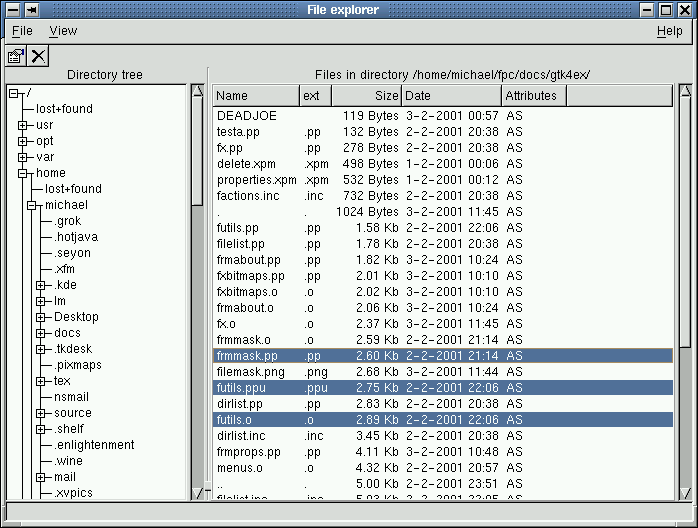
\epsfig{file=gtk4ex/mainwin.png,width=\textwidth}
\end{figure}

The toolbar contains a button to show the properties dialog. This dialog
will show the various properties of a file, and is discussed in the next
section.

\section{Adding some dialogs}
Adding some dialogs to the file explorer program is not so difficult.
Three are created, an about dialog, a file properties dialog, and a dialog
that allows to enter a file mask which will then be applied to the file
view. All three dialogs will be based on the standard GTK dialog.

Adding a dialog that shows the properties of a file is quite easy. 
The standard GTK dialog widget contains 3 widgets; a vertical box 
(\lstinline|vbox|) which can be used to drop widgets in, a separator 
and a horizontal box (\lstinline|action_area|), which can be used to 
put buttons (such as an 'OK' button) in.

The file properties dialog consists mainly of a table packed with labels and
some checkboxes. It is created in the following function:
\begin{lstlisting}{}
Type
  TFilePropertiesDialog = Record
    Window : PgtkDialog;
    Table  : PGtkTable;
    OkButton : PGtkButton;
    Labels : Array[0..1,0..NrTableLines] of PGtkLabel;
    CheckBoxes : Array[CheckBoxLineStart..NrTableLines] of PgtkCheckButton;
  end;
  PFilePropertiesDialog = ^TFilePropertiesDialog;
  
Function NewFilePropertiesDialog(FileName : String) : PFilePropertiesDialog;
Const 
  CheckAttrs : Array [CheckBoxLineStart..NrTableLines] of Integer 
             = (faReadOnly,faArchive,faHidden,faSysFile);

Var 
  Info : TSearchRec;
  I : Longint;
  
begin
  Result:=New(PFilePropertiesDialog);
  With Result^ do
    begin
    Window:=PgtkDialog(gtk_dialog_new);
    gtk_window_set_title(PgtkWindow(Window),SPropsTitle);
    gtk_window_set_modal(PgtkWindow(Window),True);
    gtk_window_set_policy(PgtkWindow(Window),0,0,0);
    gtk_window_set_position(PGtkWindow(Window),GTK_WIN_POS_CENTER);
    OkButton:=PGtkButton(gtk_button_new_with_label(SOK));
    gtk_box_pack_start(PgtkBox(Window^.action_area),PGtkWidget(Okbutton),False,False,5);
    gtk_window_set_focus(PGtkWindow(Window),PGtkWidget(OkButton));
    gtk_widget_show(PGtkWidget(OkButton));
\end{lstlisting}
The above are standard things: The dialog window title is set, the dialog is
made modal, the resizing of the window is prohibited with the
\lstinline|gtk_window_set_policy| call. Then the window is told that it
should position itself in the center of the screen with the
\lstinline|gtk_window_set_position| call. The position specifier can be one
of the following:
\begin{description}
\item[GTK\_WIN\_POS\_NONE] The window manager will decide where the window
goes.
\item[GTK\_WIN\_POS\_CENTER] The window is placed at the center of the
screen.
\item[GTK\_WIN\_POS\_MOUSE] The window is placed where the mouse cursor is.
\end{description}
After the window properties have been set, an OK button is placed in the
action area, and it gets the focus.

Next, a table is created with \lstinline|NrTableLines+1| rows and 2 columns,
and put in the vbox area:
\begin{lstlisting}{}
Table:=PgtkTable(gtk_table_new(NrTableLines+1,2,TRUE));
gtk_box_pack_start(PGtkBox(Window^.vbox),PGtkWidget(Table),True,True,10);
\end{lstlisting}
Then the table is filled with labels that describe the various properties;
the left column contains labels that simplu
\begin{lstlisting}{}
For I:=0 to NrTableLines do
  begin 
  Labels[0,i]:=PGtkLabel(gtk_label_new(LabelTexts[i]));
  gtk_label_set_justify(Labels[0,I],GTK_JUSTIFY_RIGHT);
  gtk_table_attach_defaults(Table,PgtkWidget(Labels[0,I]),0,1,I,I+1); 
  end;
For I:=0 to CheckboxLineStart-1 do
  begin 
  Labels[1,i]:=PGtkLabel(gtk_label_new(''));
  gtk_label_set_justify(Labels[1,I],GTK_JUSTIFY_LEFT);
  gtk_table_attach_defaults(Table,PgtkWidget(Labels[1,I]),1,2,I,I+1); 
  end;
\end{lstlisting}
The file attributes will be represented with checkboxes:
\begin{lstlisting}{}
For I:=CheckboxLineStart to NrTableLines do
  begin
  checkBoxes[i]:=PgtkCheckButton(gtk_check_button_new_with_label(CheckBoxTexts[I]));
  gtk_widget_set_state(PGtKWidget(CheckBoxes[i]),GTK_STATE_INSENSITIVE);
  gtk_table_attach_defaults(Table,PgtkWidget(CheckBoxes[i]),1,2,I,I+1); 
  end;  
\end{lstlisting}
The checkboxes are made inactive, so the user cannot change them.

After all labels and checkboxes are put in place, the file information
is put into various places:
\begin{lstlisting}{}
gtk_label_set_text(Labels[1,0],PChar(ExtractFileName(FileName)));
gtk_label_set_text(Labels[1,1],PChar(ExtractFilePath(FileName)));
gtk_label_set_text(Labels[1,2],PChar(ExtractFileExt(FileName)+SFile));
If FindFirst(FileName,faAnyFile,Info)=0 Then
  begin
  gtk_label_set_text(Labels[1,3],PChar(FileSizeToString(Info.Size)));
  gtk_label_set_text(Labels[1,4],PChar(DateTimeToStr(FileDateToDateTime(Info.Time))));
  For I:=CheckboxLineStart to NrTableLines do
    If (CheckAttrs[i] and Info.Attr)=CheckAttrs[i] then
      gtk_toggle_button_set_active(PgtkToggleButton(CheckBoxes[I]),True);
  FindClose(Info);
  end;
\end{lstlisting}
Finally, the 'destroy' callback for the window is set, and the OK button's
'click' signal is attached to the destroy method of the window widget:
\begin{lstlisting}{}
  gtk_signal_connect(PGtkObject(Window),'destroy',
                     TGTKSignalFunc(@DestroyPropDialog),Result);
  gtk_signal_connect_object(PgtkObject(OKButton),'clicked',
                            GTK_SIGNAL_FUNC(@gtk_widget_destroy),
                      PGTKOBJECT(Window));
  end;    
end;
\end{lstlisting}
Showing the properties dialog is simple:
\begin{lstlisting}{}
Procedure ShowFilePropertiesDialog(Dialog : PFilePropertiesDialog);

begin
  gtk_widget_show_all(PgtkWidget(Dialog^.Window));
end;
\end{lstlisting}

The result of all this is shown in figure \ref{fig:fileprops}.
\begin{figure}[ht]
\begin{center}
\caption{The file properties dialog.}\label{fig:fileprops}
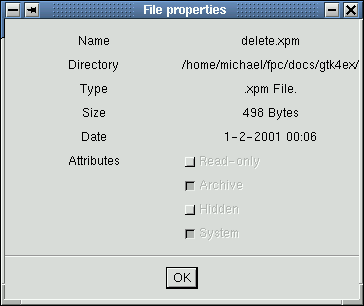
\epsfig{file=gtk4ex/fileprops.png,width=8cm}
\end{center}
\end{figure}

The handling of the mask form is a little bit more complicated than the
properties dialog, since the mask form should return some information
to the main form. 

The creation of the mask form is again a standard matter, and the reader 
is referred to the code on the CD-ROM to see how it is handled. The
only thing worth noting is the handling of the click on the 'OK' button that
appears on the form.
\begin{lstlisting}{}
gtk_signal_connect(PgtkObject(OKButton),'clicked',
                   TGtkSignalFunc(@ApplyMask),Result);
gtk_signal_connect_object(PgtkObject(OKButton),'clicked',
                   GTK_SIGNAL_FUNC(@gtk_widget_destroy),
                   PGTKOBJECT(Window));                                      
\end{lstlisting}
Two handlers are added to the 'clicked' signal of the 'OK' button.
The first one is pointed to a function that will apply the mask, and the
second one is redirected to the destroy method of the dialog window wigdet.
\begin{lstlisting}{}
Procedure ApplyMask(Widget : PGtkWidget; Window : PMaskForm);cdecl;
 
begin
With Window^ do
  begin
  Mask:=StrPas(gtk_entry_get_text(EMask));
  If (CallBack<>Nil) then
    CallBack(Mask,CallBackData);
  end;
end;
\end{lstlisting}
The \lstinline|TMaskForm| record that contains fields for all widgets on
the mask entry form also contains 2 fields that allow the OK button to notify 
the calling program of the new mask:
\begin{lstlisting}{}
  TMaskCallBack = Procedure (Mask : String; Data : Pointer);
  TMaskForm = Record
    { ... widget fields ... }
    Mask : ShortString;
    CallBack : TMaskCallBack;
    CallBackData : Pointer;
  end;
  PMaskForm = ^TMaskForm;                                                       
\end{lstlisting}
If the callback field is set, then the \lstinline|ApplyMask| function will call
it and pass it the new mask and some arbitrary pointer.

The main form contains a 'file mask' menu item, which has the following
'click' handler:
\begin{lstlisting}{}
procedure DoMask(Widget : PGtkWidget ; MainForm : PMainWindow ); cdecl;
 
Var
  S : AnsiString;
 
begin
  With NewMaskForm^ do
    begin
    S:=MainForm^.FMask;
    gtk_entry_set_text(EMask,PChar(S));
    CallBack:=@ApplyMask;
    CallBackData:=MainForm;
    gtk_widget_show_all(PgtkWidget(Window));
    end;
end;   
\end{lstlisting}
When the user clicks the 'file mask' menu item, A mask entry form is created.
The current file mask is filled in the entry widget (\lstinline|EMask|).
The callback is set, and the callbackdata is set to the pointer to the main
window record. The callback that is executed when the user clicks the OK
button on the mask form is the following:
\begin{lstlisting}{}
Procedure ApplyMask(Mask : String; Data : Pointer);
 
begin
  PMainWindow(data)^.FMask:=Mask;
  RefreshFileView(PMainWindow(Data));
end;
\end{lstlisting} 

The reason that this system of callbacks is needed is that the
\lstinline|gtk_widget_show_all| immediatly returns when the mask entry form is 
shown. Even though the mask entry form dialog is a modal dialog (i.e. it alone will
respond to mouse clicks and key presses) the call returns immediatly,
there is no counterpart for the Delphi \lstinline|ShowModal| function.

When the \lstinline|gtk_widget_show_all| returns, the mask entry form is still on
the screen, so the changes made in the mask form must be communicated 
back to the main form by means of a callback which is executed when 
the mask entry form is closed.

The mask form in action is shown in figure \ref{fig:filemask}.
\begin{figure}[ht]
\begin{center}
\caption{The file properties dialog.}\label{fig:filemask}
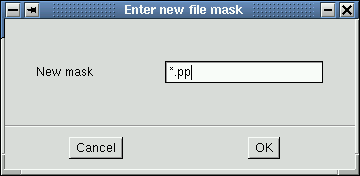
\epsfig{file=gtk4ex/filemask.png,width=8cm}
\end{center}
\end{figure}

\section{Finishing the application}
In several places in this article, a reference was made to the main menu. 
The main menu is created in the \lstinline|NewMainMenu| function; since
menus were discussed extensively in the previous article on programming GTK,
the code will not be presented here. The various calls developed in the
previous article have been collected in the \file{menus} unit. One
additional call was added which adds a check menuitem to a menu; the call is
similar to the regular menu item calls, and will not be discussed here.

The application is built in such a way that it can easily be extended. 
Only 2 file actions have been implemented, but many more can be made.
Missing functionality includes:
\begin{itemize}
\item Renaming of files. The CList allows to put an arbitrary widget into
a cell; this functionality could be used to allow the user to change the
filename by simply editing it.
\item Moving and copying of files, using drag and drop.
\item Duplicating the main window, or spawning a new window.
\item Opening a file in another application.
\item Improve the look of the file properties form.
\item On Windows, support for showing different drives should be added.
\end{itemize}
And without doubt, many more can be found.

\end{document}